\documentclass{article}

\usepackage{amsmath, amsfonts, amsthm, amssymb} 
\usepackage{listings}
\usepackage{graphicx}
\usepackage{float}
\usepackage{subfigure}
\usepackage{geometry}
\usepackage{hyperref}
\usepackage[parfill]{parskip} % no newline indent
\usepackage{enumitem} % enumerate / ordered list
\usepackage{booktabs} % three-line table
\usepackage{array}   % for \newcolumntype macro
\usepackage{listings} % MATLAB code block
\newcolumntype{C}{>{$}c<{$}} % math-mode version of "l" column type

\theoremstyle{definition} % difinition
\newtheorem{definition}{Definition}[section]
\newtheorem{theorem}{Theorem}[section]
\newtheorem{remark}{Remark}[section]

\newcommand{\dd}{\mathrm{d}}
\newcommand{\RR}{\mathbb{R}}
\newcommand{\NN}{\mathbb{N}}
\newcommand{\ZZ}{\mathbb{Z}}
\newcommand{\CC}{\mathbb{C}}
\newcommand{\PP}{\mathbb{P}}


\lstset{
  language=Matlab,  %代码语言使用的是matlab
  frame=shadowbox, %把代码用带有阴影的框圈起来
  numbers=left, % 显示行号
  breaklines=true
}

\geometry{
	paper=a4paper, 
	top=2.5cm,
	bottom=2.5cm, 
	left=2.5cm, 
	right=3cm,
	headsep=0.75cm, 
}
\title{ROB 501 HW7}
\author{Yulun Zhuang \\ \href{mailto:yulunz@umich.edu}{yulunz@umich.edu}}
\date{\today}

\begin{document}

\maketitle

\section{}
Prove, for a matrix $A\in \RR ^{m\times n}$, $rank(A) + nullity(A) = n$.

\begin{proof}
    Assume $rank(A) = r$, $\forall x\in N(A),\ Ax=0$.\\
    $\Rightarrow$ Rows of $A$ is orthogonal to $x$\\
    $\Rightarrow$ Columns of $A^T$ is orthogonal to $x$\\
    $\Rightarrow$ All $x\in N(A)$ are orthogonal to $y\in R(A^T)$\\
    $\Rightarrow$ $N(A) = R(A^T)^\perp $\\
    $\Rightarrow$ $N(A) + R(A^T) = \RR^n$ and $N(A) \cap R(A^T)^\perp = \{0\}$\\
    $\Rightarrow$ $dim(N(A)) + dim(R(A^T)) = n$\\
    $\Rightarrow$ $nullity(A) + rank(A) = n$
\end{proof}



\section{}

\begin{align*}
	A &= 
	\begin{bmatrix}
		2 & -1 & 0\\
		-1 & 2 & 1\\
		0 & 1 & 2
	\end{bmatrix}
	\\
	&=
	\begin{bmatrix}
		-0.5 & 0.707 & 0.5\\
		-0.707 & 0 & -0.707\\
		0.5 & 0.707 & -0.5
	\end{bmatrix}
	\begin{bmatrix}
		0.586 & 0 & 0\\
		0 & 2 & 0\\
		0 & 0 & 3.414
	\end{bmatrix}
	\begin{bmatrix}
		-0.5 & 0.707 & 0.5\\
		-0.707 & 0 & -0.707\\
		0.5 & 0.707 & -0.5
	\end{bmatrix}
	\\
	&=O \Lambda O^T
\end{align*}

\section{}
\begin{align*}
	O^T A O = diag([2, -1, 2])
\end{align*}

\section{}

\subsection{}
Find $n=34$.

\subsection{}
\begin{figure}[H]
    \centering
        \textsf{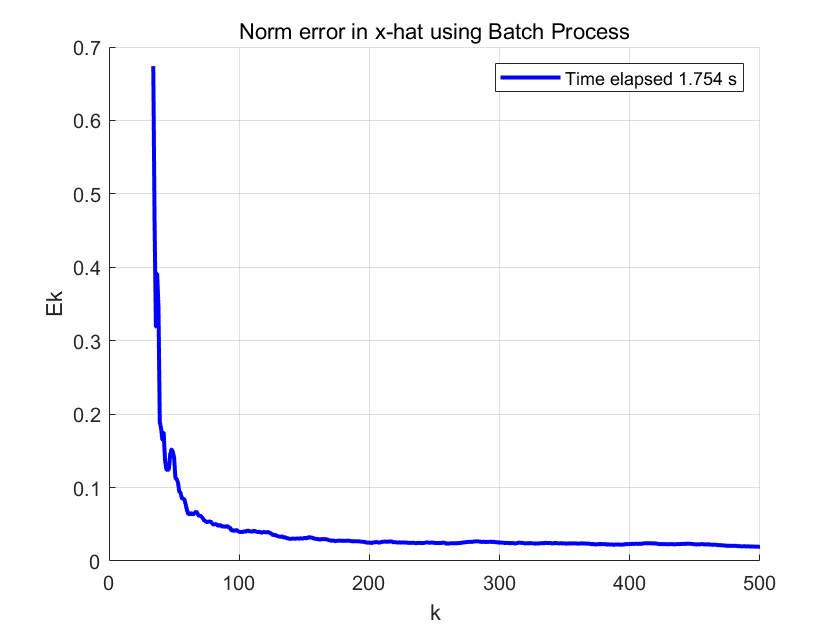
\includegraphics[width=0.6\columnwidth]{HW7-prob4-fig1.png}}
        \caption{Norm error in x-hat using Batch Process}
        \label{fig: 4-1}
\end{figure}

\subsection{}
\begin{figure}[H]
    \centering
        \textsf{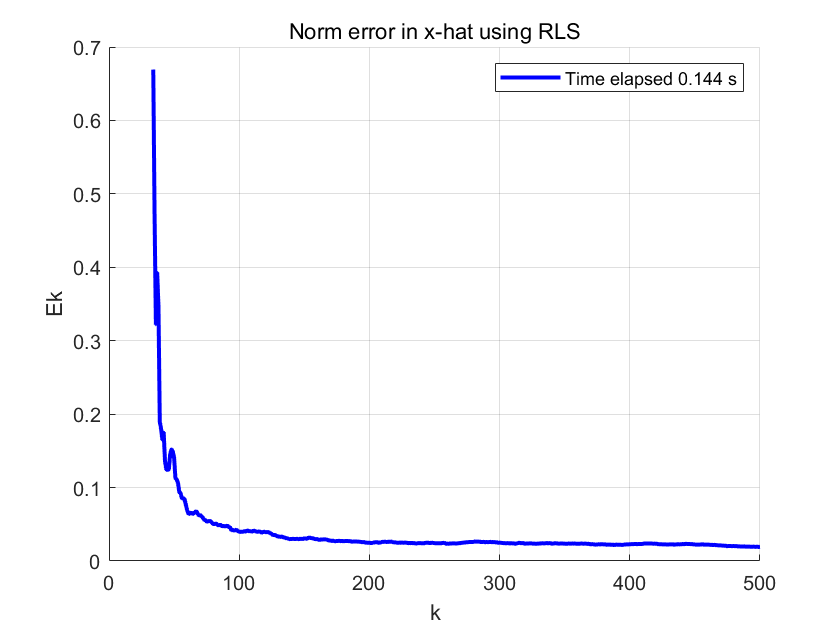
\includegraphics[width=0.6\columnwidth]{HW7-prob4-fig2.png}}
        \caption{Norm error in x-hat using Recursive Least Squares (RLS)}
        \label{fig: 4-2}
\end{figure}

\subsection{}
\begin{figure}[H]
    \centering
        \textsf{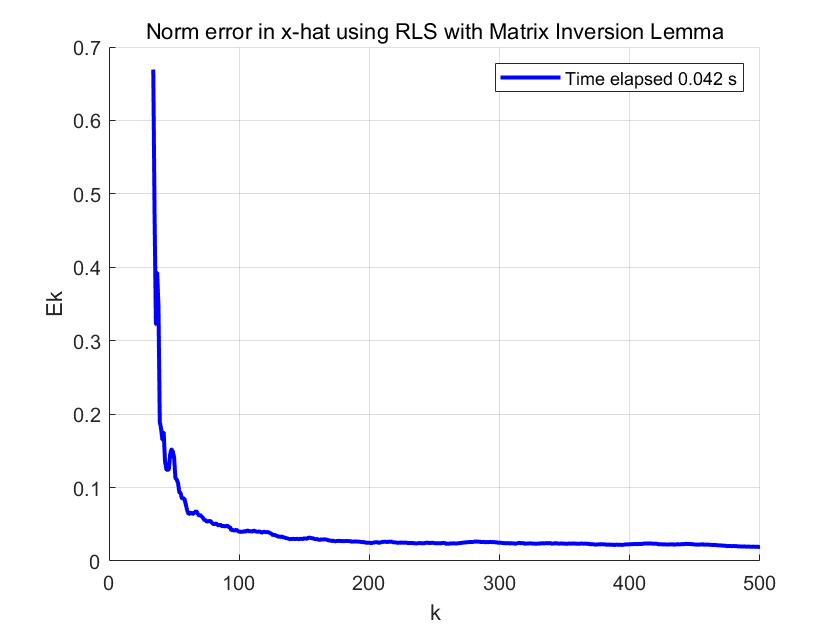
\includegraphics[width=0.6\columnwidth]{HW7-prob4-fig3.png}}
        \caption{Norm error in x-hat using RLS with Matrix Inversion Lemma}
        \label{fig: 4-3}
\end{figure}

\section{}
\subsection{}
Find $n=7$.

\subsection{}
\begin{figure}[H]
    \centering
        \textsf{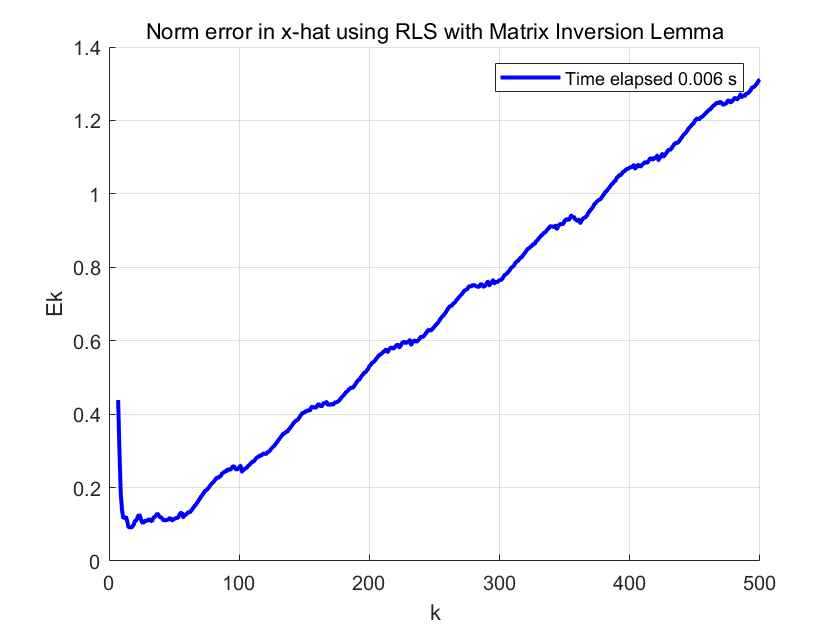
\includegraphics[width=0.6\columnwidth]{HW7-prob5-fig1.png}}
        \caption{Norm error in x-hat using RLS with Matrix Inversion Lemma}
        \label{fig: 5-1}
\end{figure}

\subsection{}
\begin{figure}[H]
    \centering
        \textsf{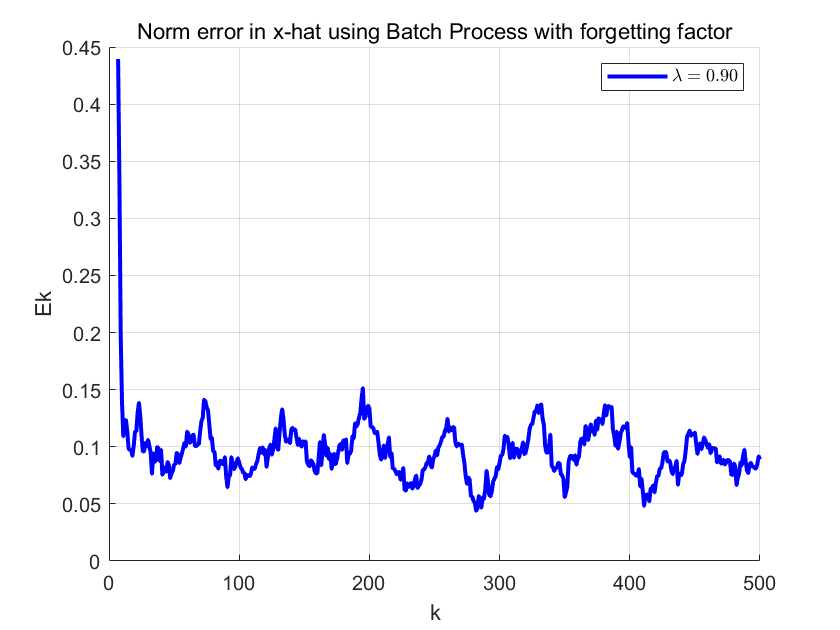
\includegraphics[width=0.6\columnwidth]{HW7-prob5-fig2.png}}
        \caption{Norm error in x-hat using Batch Process with forgetting factor}
        \label{fig: 5-2}
\end{figure}

\subsection{}
\begin{figure}[H]
    \centering
        \textsf{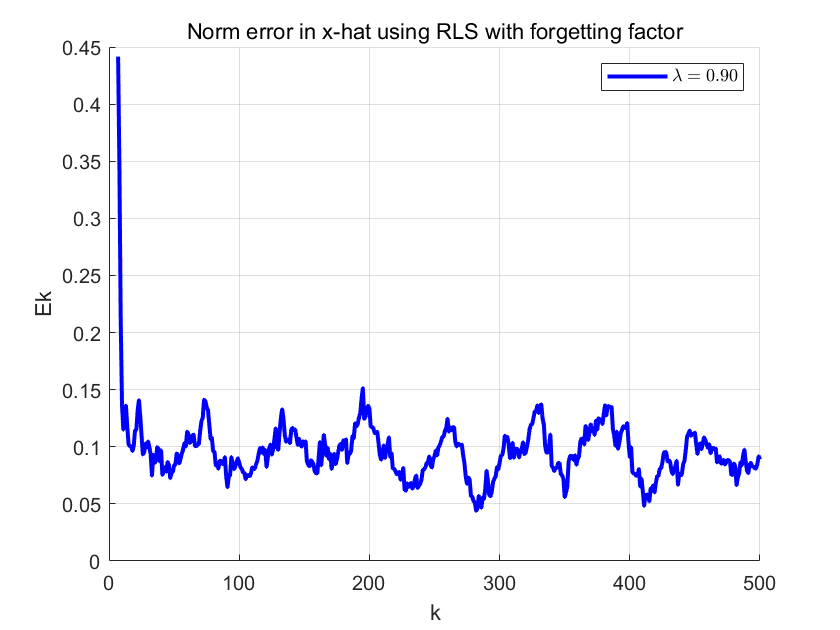
\includegraphics[width=0.6\columnwidth]{HW7-prob5-fig3.png}}
        \caption{Norm error in x-hat using RLS with forgetting factor}
        \label{fig: 5-3}
\end{figure}

\section{}
\subsection{}

\begin{align*}
	A &=
	\begin{bmatrix}
		1 & 3\\ 3 & 9
	\end{bmatrix}, \text{e-values: 10, 0}
	\\
	\Rightarrow A & \text{ is positive semi-definite.}
	\\
	A & = O\Lambda O^T \\
	&= O\Lambda^{\frac{1}{2}T} \Lambda^{\frac{1}{2}} O^T\\
	&= (\Lambda^{\frac{1}{2}} O^T)^T(\Lambda^{\frac{1}{2}} O^T)\\
	\Rightarrow \Lambda^{\frac{1}{2}} &O^T = 
	\begin{bmatrix}
		0 & 0 \\ 1 & 3
	\end{bmatrix}
\end{align*}

\subsection{}

\begin{align*}
	B &=
	\begin{bmatrix}
		6 & 10 & 11\\
		10 & 19 & 19\\
		11 & 19 & 21
	\end{bmatrix}, \text{e-values: 0.1856, 1.0842, 44.7302}
	\\
	\Rightarrow B & \text{ is positive definite.}
	\\
	B & = O\Lambda O^T \\
	&= (\Lambda^{\frac{1}{2}} O^T)^T(\Lambda^{\frac{1}{2}} O^T)\\
	\Rightarrow \Lambda^{\frac{1}{2}} &O^T = 
	\left[\begin{array}{ccc}
		-0.3767 & -0.0105 & 0.2087 \\
		0.3405 & -0.7991 & 0.5743 \\
		2.3963 & 4.2850 & 4.5417
	\end{array}\right]
\end{align*}

\subsection{}

\begin{align*}
	C &=
	\begin{bmatrix}
		2 & 6 & 10\\
		6 & 10 & 14\\
		10 & 14 & 18
	\end{bmatrix}, \text{e-values: -2.9165, 0, 32.9165}
	\\
	\Rightarrow C & \text{ is neigher positive definite or positive semi-definite.}
\end{align*}

\section{}

Recall the Schur Complements: suppose that $A$, $B$ and $C$ are real matrices, $A\in \RR^{n\times n}$ is symmetric, $B\in \RR ^{n\times m}$, and $C\in \RR^{m\times m}$ is symmetric. We have

$$
M = 
\begin{bmatrix}
	A & B \\ B^T & C
\end{bmatrix}
$$

the following statements are equivalent:

(a) $M>0$.\\
(b) $A>0$, and $C-B^{\top} A^{-1} B>0$.\\
(c) $C>0$, and $A-B C^{-1} B^{\top}>0$.

\subsection{}

$$
\begin{aligned}
&A_1 =\left[\begin{array}{ll}
1 & 3 \\
3 & 8
\end{array}\right] \\
&A =1>0 \\
&C-B^{\top} A^{-1} B =8-3 \times 1 \times 3 = -1<0\\
\Rightarrow &A_1  \text{ is not positue definite}
\end{aligned}
$$

\subsection{}
\begin{align*}
	&A_2=\left[\begin{array}{lll}
	1 & 0 & 6 \\
	0 & 4 & 7 \\
	6 & 7 & 10
	\end{array}\right]\\
	&\text {Let } A=\left[\begin{array}{ll}
	1 & 0 \\
	0 & 4
	\end{array}\right], B=\left[\begin{array}{l}
	6 \\
	7
	\end{array}\right], \quad C=10\\
	&C=10>0\\
	&A-B C^{-1} B^{\top}=
	\left[\begin{array}{ll}
	1 & 0 \\
	0 & 4
	\end{array}\right]
	-
	\frac{1}{10}\left[\begin{array}{l}
	6 \\
	7
	\end{array}\right]\left[\begin{array}{ll}
	6 & 7
	\end{array}\right]\\
	% &=\left[\begin{array}{ll}
	% 1 & 0 \\
	% 0 & 4
	% \end{array}\right]-\left[\begin{array}{ll}
	% 3.6 & 4.2 \\
	% 4.2 & 4.9
	% \end{array}\right]\\
	&=\left[\begin{array}{ll}
	-2.6 & -4.2 \\
	-4.2 & -0.9
	\end{array}\right]
	<0\\
	\Rightarrow &{A}_2 \text { is not positive definite }
\end{align*}

\subsection{}
\begin{align*}
	&A_3=\left[\begin{array}{lll}
	1 & 2 & 6 \\
	2 & 5 & 7 \\
	6 & 7 & a
	\end{array}\right] \\
	&\text {Let } A=\left[\begin{array}{ll}
	1 & 2 \\
	2 & 5
	\end{array}\right], B=\left[\begin{array}{l}
	6 \\
	7
	\end{array}\right], C=a \\
	&\left\{\begin{array}{l}
	C>0 \\
	A-B C^{-1} B^{\top}>0
	\end{array}\right.\\
	\Rightarrow\ &a>0 \text{ and }\\
	&\left[\begin{array}{ll}
	1 & 2 \\
	2 & 5
	\end{array}\right]-\frac{1}{a}\left[\begin{array}{ll}
	36 & 42 \\
	42 & 49
	\end{array}\right]>0\\
	&\left[\begin{array}{cc}
	1-36/a & 2-42/a \\
	2-42/a & 5-49/a
	\end{array}\right]>0\\
	&\text {Let } A=1-\frac{36}{a}, B=2-\frac{42}{a}, C=5-\frac{49}{a} \\
	&\left\{\begin{array}{l}
	A>0 \\
	C-B^{\top} A^{-1} B>0
	\end{array}\right.\\
	\Rightarrow\ &a>36  \text{ and }\\
	&5-\frac{49}{a}-\left(2-\frac{42}{a}\right) \frac{a}{a-36}\left(2-\frac{42}{a}\right)>0 \\
	% &5-\frac{49}{a}-\left(4-\frac{168}{a}+\frac{42^2}{a^2}\right) \frac{a}{a-36}>0 \\
	&5 a-49-\frac{4 a^2-168 a+42^2}{a-36}>0 \\
	&(5 a-49)(a-36)>4 a^2-168 a+42^2 \\
	% &5 a^2-229+1764>4 a^2-168 a+1764 \\
	&a^2-61 a>0 \\
	\Rightarrow\ &a<0  \text { or }  a>61
\end{align*}
Hence, $a>61$.


\section{}
Given 
$$
A=\left[\begin{array}{lll}
1 & 3 & 2 \\
3 & 8 & 4
\end{array}\right],\ b=\left[\begin{array}{l}
1 \\
2
\end{array}\right]
$$
Find the minimum norm solution $x$, s.t. $A x=b$

\subsection{}

$$
\tilde{x}=A^{\top}\left(A A^{\top}\right)^{-1} b=
\left[\begin{array}{c}
	-0.0952 \\ 0,0476 \\ 0.4762
\end{array}\right]
$$

\subsection{}
Let $M=\left[\begin{array}{lll}5 & 1 & 9 \\ 1 & 2 & 1 \\ 9 & 1 & 17\end{array}\right]$, note that $M$ is symmetric with $M=M^{\top}$ under the inner product convension $\langle x, y\rangle=x^{\top} M y$.

Denote the least norm solution as $x_{\ln}$. We find $x{\ln}$ as the solution of a constrained optimization problem.

\begin{align*}
	\min &\quad \left\|x\right\|^2 \\
	\text { s.t. } &\ A x=b
\end{align*}

Then remove the constraints using Lagrange multiplier for matrix (i.e. $\lambda \in \RR^{2}$ and $\lambda > 0$).

\begin{align*}
	&L(x)= x^{\top} M x-\lambda^{\top}\left(A x-b\right) \\
	&\nabla L(x)= 2 x^{\top} M-\lambda^{\top} A\\
	&\left\{\begin{array}{l}2 x^{\top} M-\lambda^{\top} A=0 \\ A x-b = 0\end{array}\right.\\
	&x=\frac{1}{2} M^{-1} A^{\top} \lambda\\
	&\frac{1}{2} \underbrace{A M^{-1} A^{\top}}_{\text {invertible}} \lambda=b\\
	&\lambda=2\left(A M^{-1} A^{\top}\right)^{-1} b\\
	\Rightarrow\ &x_{\ln}=M^{-1} A^{\top}\left(A M^{-1} A^{\top}\right)^{-1} b\\
	&x_{\ln}=\left[\begin{array}{c}-0.6497 \\ 0.3248 \\ 0.3376\end{array}\right]
\end{align*}


\end{document}